\documentclass[12pt,french,letterpaper]{article}
%déclaration du document 

\usepackage[T1]{fontenc}
%package pour police
\usepackage[utf8]{inputenc}
%package pour police

\usepackage[document]{ragged2e}
\usepackage{graphicx}
\usepackage{fancyhdr}
\usepackage{biblatex}
\usepackage{csquotes}
\usepackage[svgnames]{xcolor}

\usepackage{mathptmx}%choix de la police mathptmx = Times

\usepackage[dvipsnames,svgnames]{xcolor}%chois pour les couleurs


\usepackage{float}
\let\origfigure=\figure
\let\endorigfigure=\endfigure
\renewenvironment{figure}[1][]{%
  \origfigure[H]
}{%
  \endorigfigure
}

\usepackage{epigraph}
\usepackage{fancyhdr}


\providecommand{\subtitle}[1]{}
\subtitle{Des recettes allemandes typiques avec des pommes de terre}
\author{Lili    Ricke    Université de Montréal }
\providecommand{\cours}[1]{}
\cours{FRA3825 Pratiques de l'édition numérique}
\cours{}
\date{}


\pagestyle{fancy}
\fancyhf{}
\lhead{}
\rhead{}
\cfoot{Page \thepage}

\usepackage{graphicx}%package pour la gestion des images
\graphicspath{ {./media/} }%chemin des figures

\usepackage{graphicx,grffile}
\makeatletter
\def\maxwidth{\ifdim\Gin@nat@width>\linewidth\linewidth\else\Gin@nat@width\fi}
\def\maxheight{\ifdim\Gin@nat@height>\textheight\textheight\else\Gin@nat@height\fi}
\makeatother
% Scale images if necessary, so that they will not overflow the page
% margins by default, and it is still possible to overwrite the defaults
% using explicit options in \includegraphics[width, height, ...]{}
\setkeys{Gin}{width=\maxwidth,height=\maxheight,keepaspectratio}

\usepackage{amssymb,amsmath}
\usepackage{ifxetex,ifluatex}
\usepackage{fixltx2e} % provides \textsubscript
\ifnum 0\ifxetex 1\fi\ifluatex 1\fi=0 % if pdftex
  \usepackage[T1]{fontenc}


\else % if luatex or xelatex

  \usepackage{unicode-math}

  \defaultfontfeatures{Ligatures=TeX,Scale=MatchLowercase}
\fi
% use upquote if available, for straight quotes in verbatim environments
\IfFileExists{upquote.sty}{\usepackage{upquote}}{}
% use microtype if available
\IfFileExists{microtype.sty}{%
\usepackage[]{microtype}
\UseMicrotypeSet[protrusion]{basicmath} % disable protrusion for tt fonts
}{}
\PassOptionsToPackage{hyphens}{url} % url is loaded by hyperref

\usepackage[unicode=true]{hyperref}
\hypersetup{
            pdftitle={La pomme de terre : Des recettes allemandes
typiques avec des pommes de terre},
            pdfauthor={Lili ,  Ricke,  },
            colorlinks=true,
            urlcolor= RoyalBlue, 
	          linkcolor= Gold,
            pdfborder={0 0 0},
            breaklinks=true}
\urlstyle{same}  % don't use monospace font for urls



\IfFileExists{parskip.sty}{%
\usepackage{parskip}
}{% else
\setlength{\parindent}{0pt}
\setlength{\parskip}{6pt plus 2pt minus 1pt}
}
\setlength{\emergencystretch}{3em}  % prevent overfull lines
\providecommand{\tightlist}{%
  \setlength{\itemsep}{0pt}\setlength{\parskip}{0pt}}
\setcounter{secnumdepth}{0}
% Redefines (sub)paragraphs to behave more like sections
\ifx\paragraph\undefined\else
\let\oldparagraph\paragraph
\renewcommand{\paragraph}[1]{\oldparagraph{#1}\mbox{}}
\fi
\ifx\subparagraph\undefined\else
\let\oldsubparagraph\subparagraph
\renewcommand{\subparagraph}[1]{\oldsubparagraph{#1}\mbox{}}
\fi

% set default figure placement to htbp
\makeatletter
\def\fps@figure{htbp}
\makeatother




\begin{document}%début de mon document

\begin{titlepage}%début de ma page de titre
\begin{center}
    \enlargethispage{2cm}
    

\includegraphics[width = 50mm]{logo} %ajout de l'image en taille logo
%si le logo ne fonctionne pas : 
%\scshape{Université de Montréal} %utilisation des small caps 

\vspace*{3cm}
\scshape\Huge La pomme de terre\\
\normalfont\Large Des recettes allemandes typiques avec des pommes de
terre\\
\large \vspace*{3cm}
Lili,  Ricke,  
\\
\normalsize\vspace*{1cm}Travail présenté dans le cadre du cours FRA3825 - \em Pratiques
de l'édition numérique
 \normalfont donné par Margot Mellet 

\vspace*{3cm}
\end{center}

\vspace*{\fill}
\begin{flushright}
\end{flushright}

\begin{center}
\scshape\normalsize\vspace*{1cm} 21-Mars-2023 --      Université de
Montréal 
\\
\end{center}
\end{titlepage}




\newpage 

\normalsize{\hypertarget{proposition-du-sujet}{%
\subsection{Proposition du sujet}\label{proposition-du-sujet}}

\textbf{Besoin d'écriture :}

J'aimerais dédier mon article à la pomme de terre. À première vue, ce
sujet peut sembler un peu étrange, mais il y a une raison très concrète
derrière ce choix de sujet. En fait, je viens d'Allemagne et on me
demande donc souvent ce que sont les plats allemands typiques. À cela,
je réponds toujours que chaque plat avec des pommes de terre est
typiquement allemand. Après cela, on me demande toujours de donner
quelques exemples et d'expliquer comment préparer ces plats. Cependant,
la plupart des personnes ne peuvent plus me suivre jusque-là parce
qu'ils ne connaissent pas du tout ces nombreux plats différents avec des
pommes de terre et ne comprennent pas ce que j'entends, par exemple, par
\href{https://fr.wikipedia.org/wiki/Galette_de_pommes_de_terre}{\emph{Kartoffelpuffer}}
et pourquoi je les aime tant.
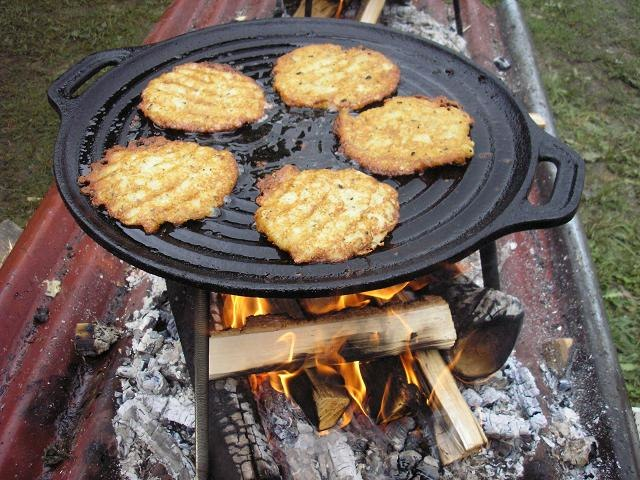
\includegraphics{/media/Kartoffelpuffer.jpg}

En outre, 19 \% des Allemands mangent de la salade de pommes de terre à
Noël et en Allemagne de l'Est, c'est même 40 \%\footnote{{[}@WarumBockwurstUnd{]}}.
En revanche, ici à Montréal, plusieurs amis sont venus me voir
complètement désemparés avec leurs pommes de terre puisqu'ils ne savent
tout simplement pas comment les préparer. Par conséquent, je voudrais
les aider avec mon article numérique et leur montrer à quel point les
recettes avec des pommes de terre sont faciles à préparer et à quel
point elles sont délicieuses. En général, j'aimerais utiliser mon projet
pour rapprocher la cuisine allemande de mes nombreux amis étrangers. Je
souhaite souligner à quel point la pomme de terre et la cuisine
allemande sont diversifiées et pourquoi nous mangeons des pommes de
terre plusieurs fois par semaine en Allemagne.

\textbf{Objectifs et Inspiration :}

Dans mon article, j'imagine présenter non seulement des recettes
allemandes typiques avec des pommes de terre, mais aussi informer sur la
pomme de terre en général. En conséquence, je discuterai de l'histoire,
de la diffusion, des formes et des couleurs de la pomme de terre. Les
blogs culinaires et les blogs d'information devraient servir
d'inspiration pour moi. Je souhaite rendre mon article très vivant,
convivial et accueillant. Afin de mettre cela en œuvre, j'aimerais
intégrer de nombreuses images, couleurs et liens qui mènent à des
informations supplémentaires. Sinon, je me référai également à des
livres de cuisine et des vidéos YouTube qui expliquent comment préparer
des plats avec des pommes de terre. De plus, une structure claire de mon
article est très importante pour moi. Mon article devrait inviter à
s'attarder, à être informatif et divertissant.

\newpage

\hypertarget{bibliographie}{%
\subsection{Bibliographie}\label{bibliographie}}

Maciarka (1899, 30 novembre). \emph{Zemiakové placky}{[}image en
ligne{]}. Wikimedia Commons.
\url{https://commons.wikimedia.org/wiki/File:Zemiakové_placky_ゼミアコベー・プラツキー.JPG}

Prof.~Berg, Renate (2021, 9 janvier). \emph{Warum bockwurst und
kartoffelsalat zu weihnachten ?} alleantworten.
\url{https://alleantworten.de/warum-bockwurst-und-kartoffelsalat-zu-weihnachten}.}



\end{document}
